\subsubsection{Overview / description/parameters}
Describe concept of accumulator pack, provide table with main parameters like number of cells, cell stacks separated by maintenance plugs, cell configuration, resulting voltages->minimum, maximum, nominal, currents, capacity etc.
Fill out the following table:

\begin{table}[H]
	\centering
	\caption{Main accumulator parameters}
	\begin{tabularx}{\textwidth}{|X|X|}
		\hline
		Maximum Voltage: & 400 VDC \\[\TableSize]
		\hline
		Nominal Voltage: & 345.6 VDC \\[\TableSize]
		\hline
		Minimum Voltage: & 182 VDC \\[\TableSize]
		\hline
		Maximum output current: & 315 A (until any cell reaches 80 $^\circ$C) \\[\TableSize]
		\hline
		Maximum nominal current: & 270 A \\[\TableSize]
		\hline
		Maximum charging current: & 54 A \\[\TableSize]
		\hline
		Total numbers of cells: & 864 \\[\TableSize]
		\hline
		Cell configuration: & 96s9p \\[\TableSize]
		\hline
		Total Capacity: & 27.99 MJ \\[\TableSize]
		\hline
		Number of cell stacks < 120VDC & 6 \\[\TableSize]
		\hline
	\end{tabularx}%
	\label{tab:acc-main}%
\end{table}%

\subsubsection{Cell description}
Describe the cell type used and the chemistry, provide table with main parameters.
Fill out the following table:

\begin{table}[H]
	\centering
	\caption{Main cell specification}
	\begin{tabularx}{\textwidth}{|X|X|}
		\hline
		Cell Manufacturer and Type & SONY VTC5A \\[\TableSize]
		\hline
		Cell nominal capacity: & 2.5 Ah \\[\TableSize]
		\hline
		Maximum Voltage: & 4.25 V \\[\TableSize]
		\hline
		Nominal Voltage: & 3.6 V \\[\TableSize]
		\hline
		Minimum Voltage:  & 2 V \\[\TableSize]
		\hline
		Maximum output current: & 35 A (until cell reaches 80 $^\circ$C) (14C)\\[\TableSize]
		\hline
		Maximum nominal output current: & 30A(12C) \\[\TableSize]
		\hline
		Maximum charging current: & 6A(2.4C) \\[\TableSize]
		\hline
		Maximum Cell Temperature (discharging) & 80 $^\circ$C \\[\TableSize]
		\hline
		Maximum Cell Temperature (charging) & 60 $^\circ$C \\[\TableSize]
		\hline
		Cell chemistry: & Lithium-Ion \\[\TableSize]
		\hline
	\end{tabularx}%
	\label{tab:acc-cell}%
\end{table}%

\subsubsection{Cell configuration}
%Describe cell configuration, cell interconnect, show schematics of electrical configuration and CAD of connection techniques, cover additional parts like internal cell fuses etc.

Cell configuration is 96s9p. Cells are divided into 6 stacks, configuration of each stack is 16s9p. Cells are connected by welding. Main cells interconnection is done by nickel sheet. This sheet is welded to each cell. There is additional copper sheet welded over the nickel sheet (for lowering resistance of the main current path).

 
\subsubsection{Cell temperature monitoring}
%Describe how the temperature of the cells is monitored, where the temperature sensors are placed, how many cells are monitored, etc. Show schematics, cover additional parts, etc.

The cells’ temperature is monitored by NTC temperature sensors. The manufacturer is TDK, type is: B57330V2103F260. Insulation of the sensors is done by 3M™ PTFE Film Electrical Tape. Breakdown voltage of this tape 9.5 kV, operating temperature is 180 $^\circ$C. Thickness of this tape is 0.1 mm. Sensors are soldered in PCBs that are covered with insulating tape and then mounted to each stack. 

\begin{figure}[H]
	\centering
	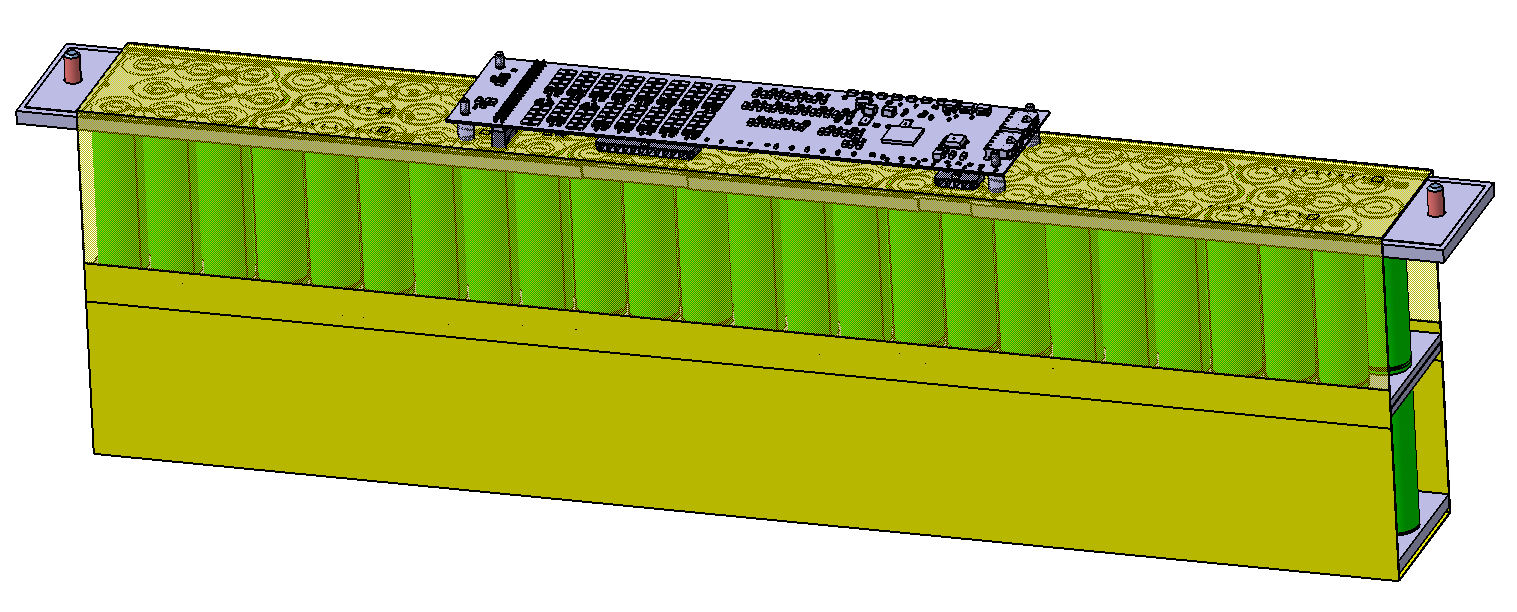
\includegraphics[width=\textwidth]{./img/ACP-stack.png}
	\caption{Stack configuration.}
	\label{fig:acp-stack}
\end{figure}

Position of temperature sensors on the top of each stack (highlighted objects)
\begin{figure}[H]
	\centering
	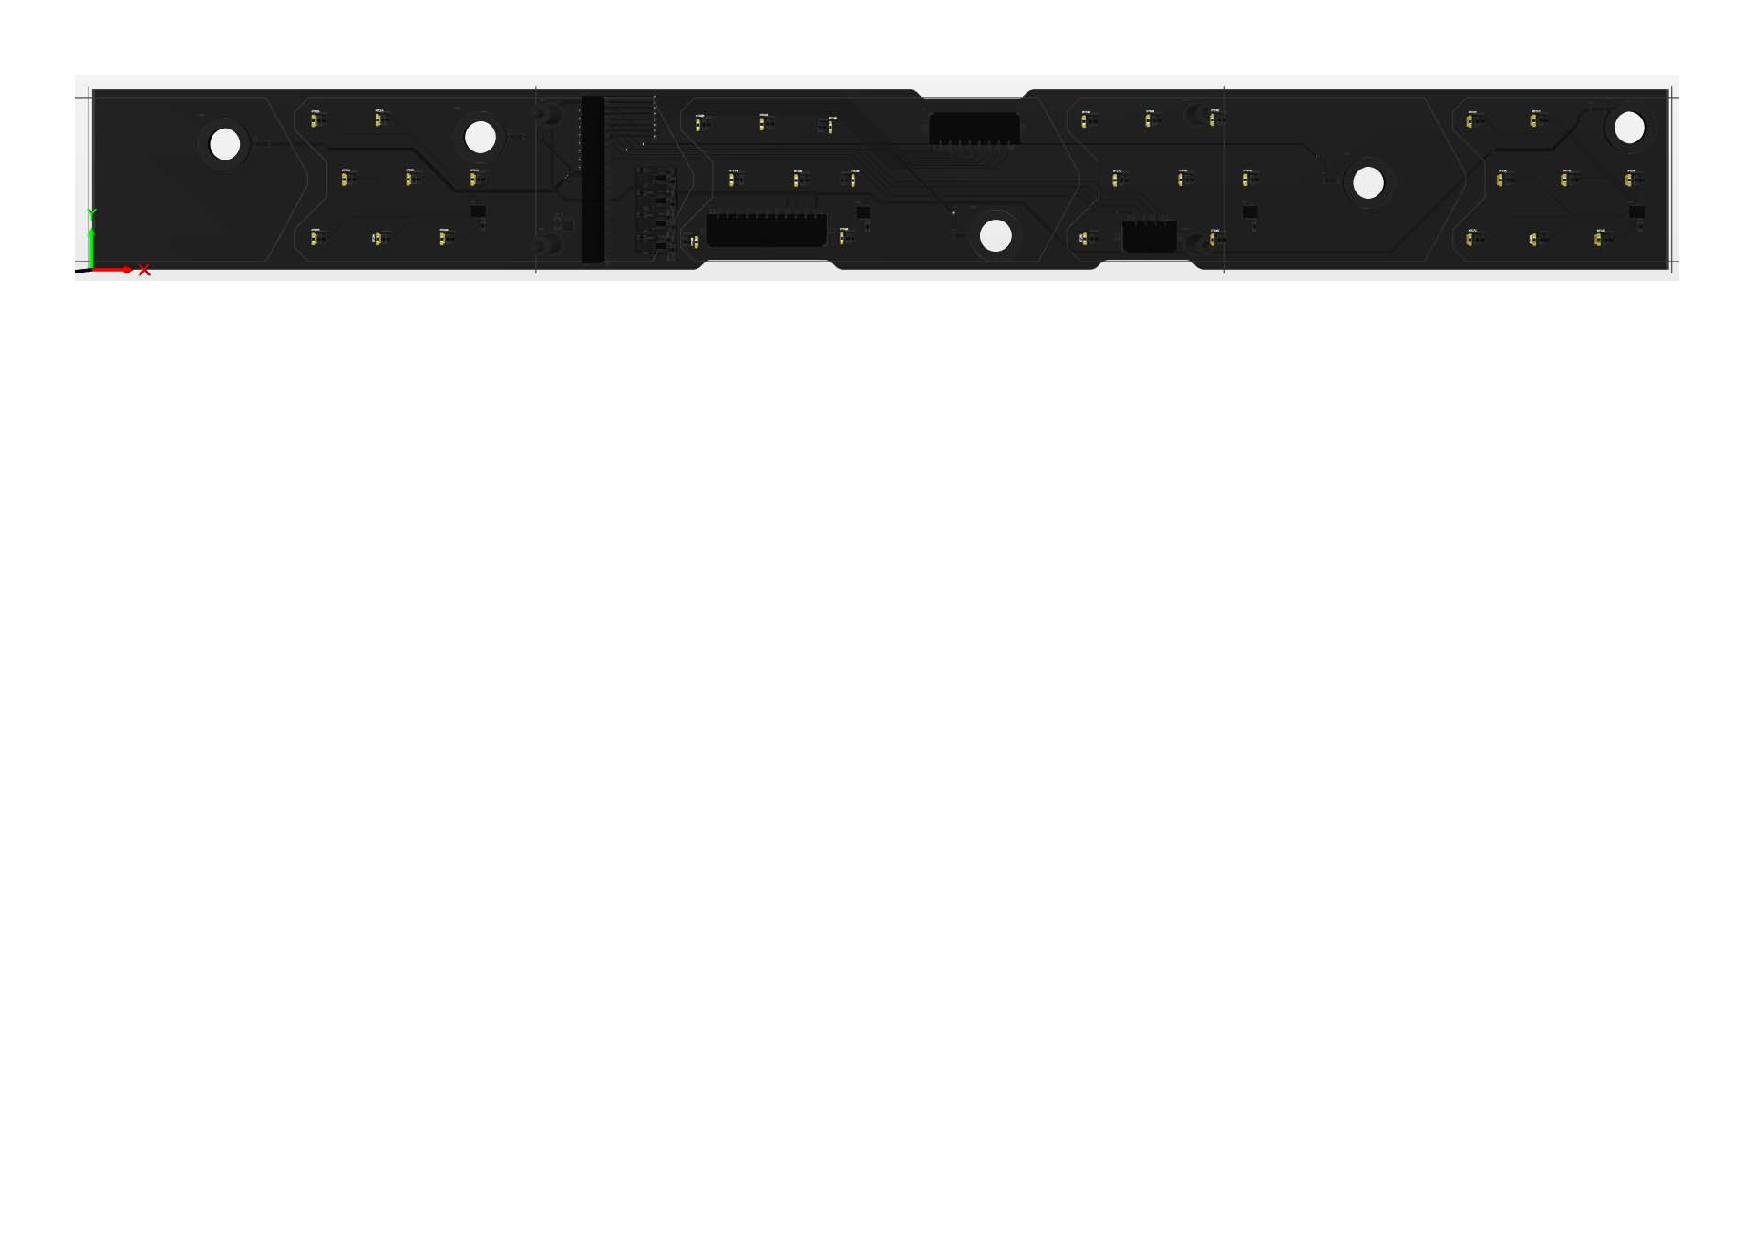
\includegraphics[width=\textwidth,trim={0cm 16cm 0cm 0cm}, clip]{./img/BMS-top-sensors.pdf}
	\caption{Top position of sensors.}
	\label{fig:BMS-top}
\end{figure}
Position of temperature sensors on the bottom of each stack (highlighted objects)
\begin{figure}[H]
	\centering
	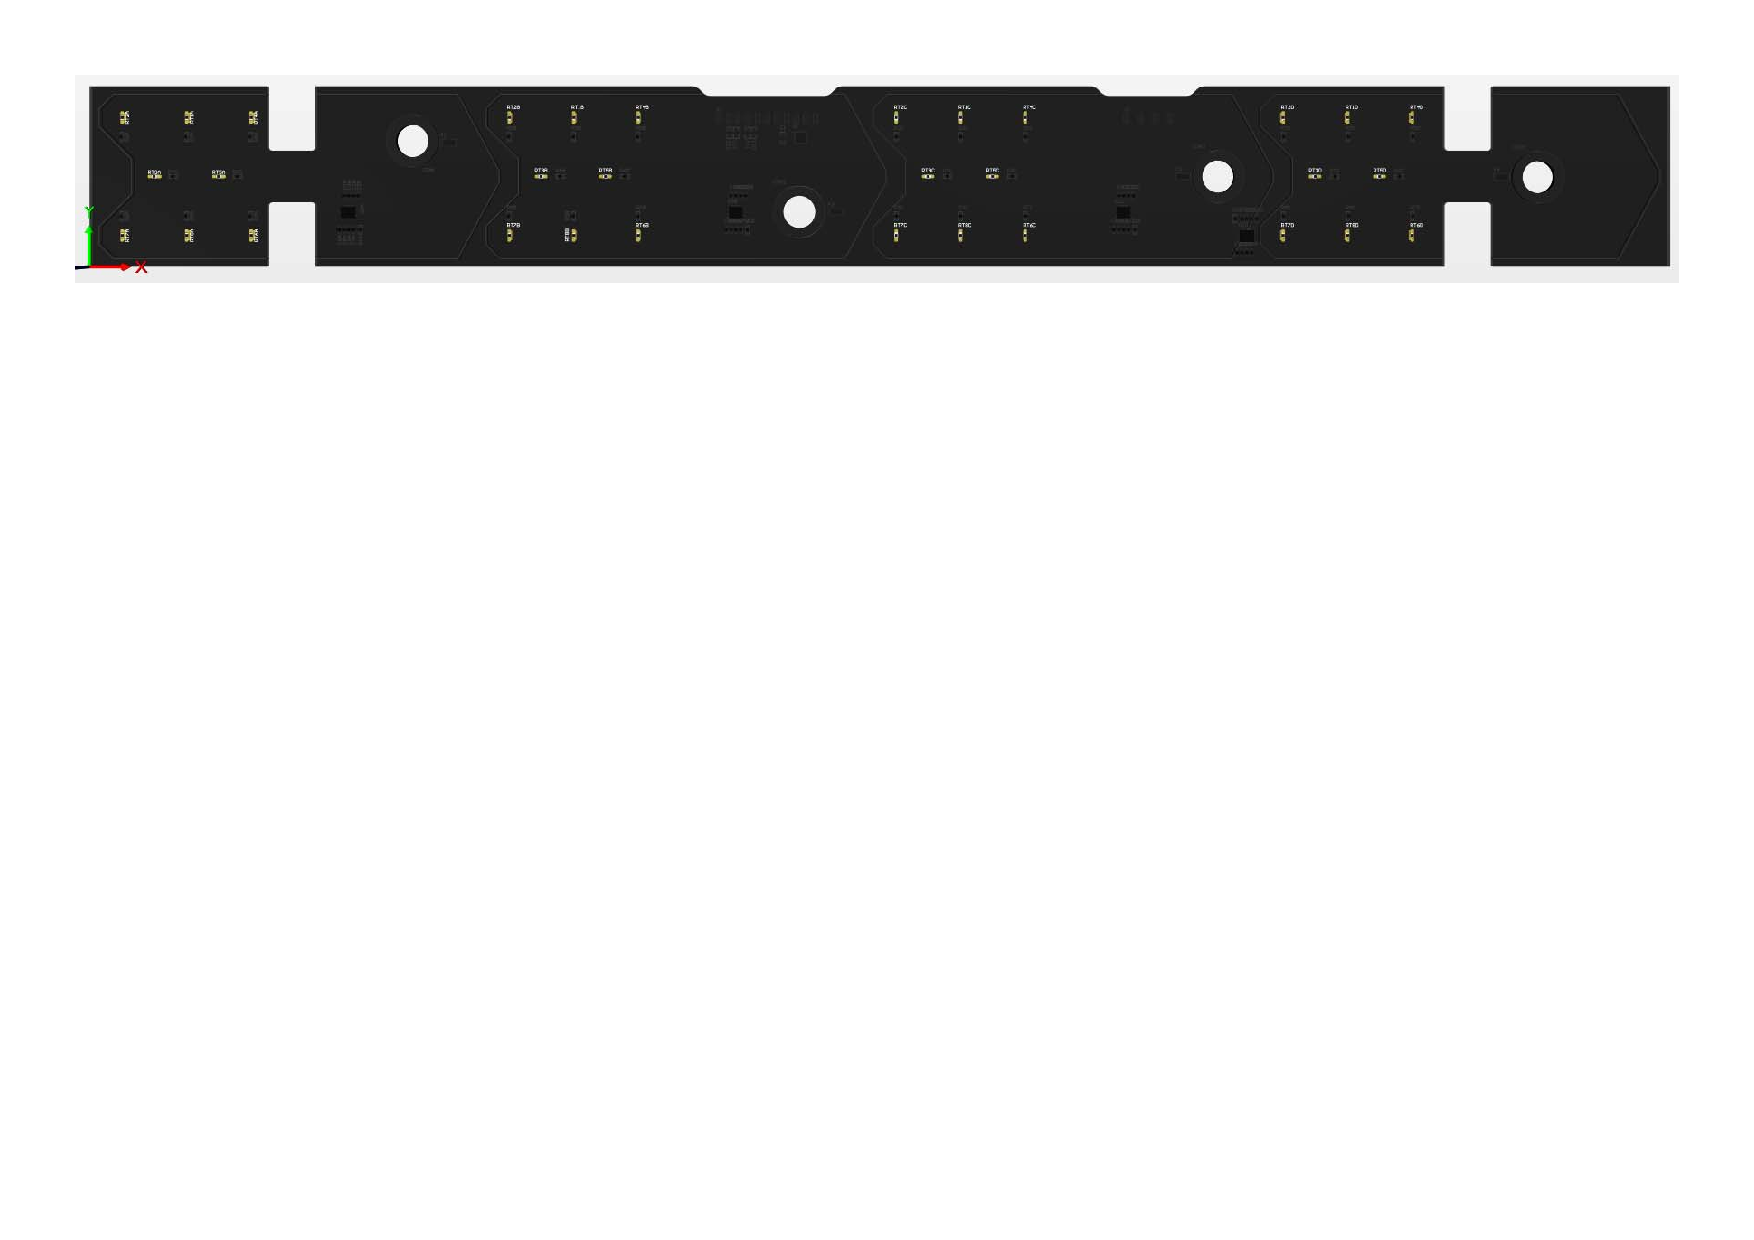
\includegraphics[width=\textwidth,trim={0cm 16cm 0cm 0cm}, clip]{./img/BMS-bottom-sensors.pdf}
	\caption{Bottom position of sensors.}
	\label{fig:bms-bottom}
\end{figure}
Top and bottom view of one stack 
\begin{figure}[H]
	\centering
	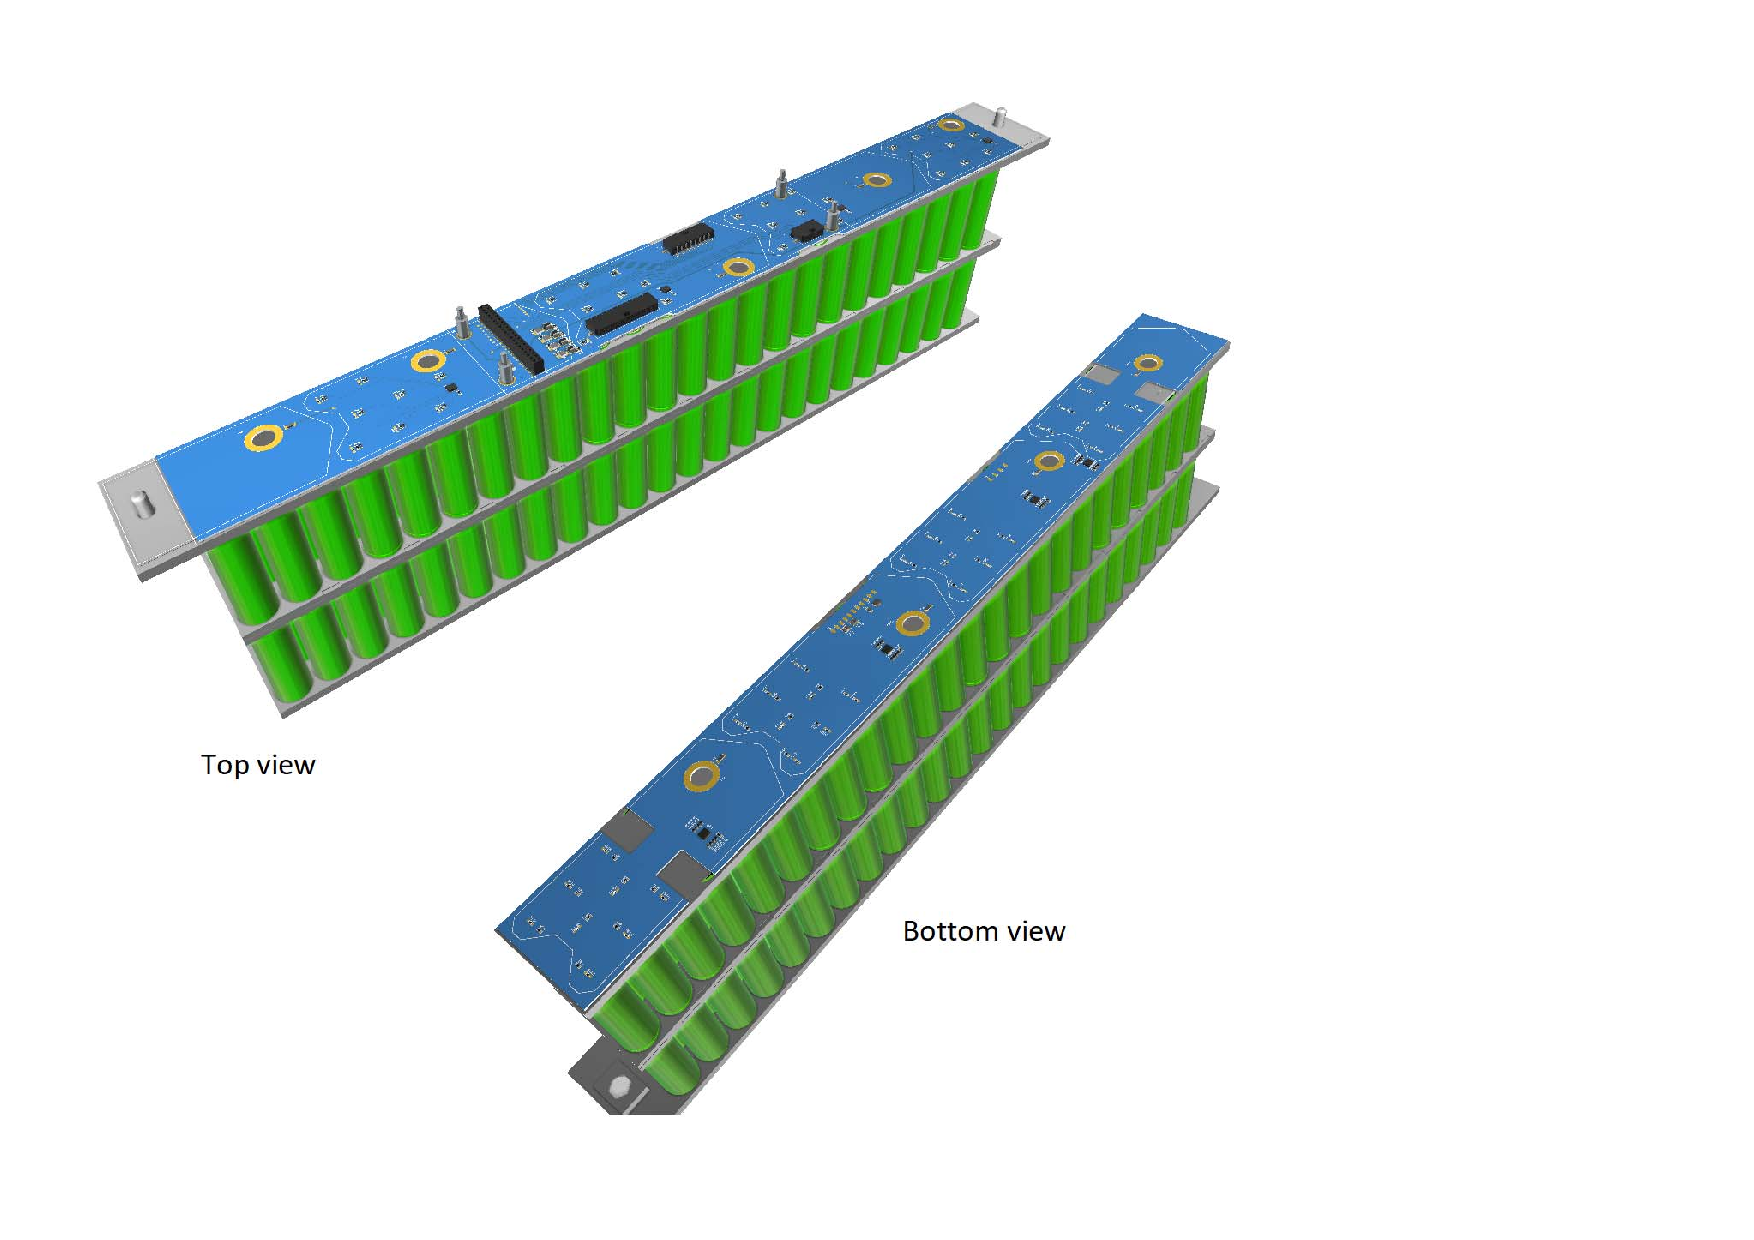
\includegraphics[width=\textwidth]{./img/BMS-top-andbottom.pdf}
	\caption{Rear and bottom view.}
	\label{fig:torque1}
\end{figure}

\begin{table}[H]
	\centering
	\caption{General cell temperature parameters.}
	\begin{tabularx}{\textwidth}{|X|X|}
		\hline
		Temperature sensor accuracy: & 1\% \\[\TableSize]
		\hline
		Total number of cells: & 864 \\[\TableSize]
		\hline
		Total number of sensors: &  384 \\[\TableSize]
		\hline
		Max. distance from monitored negative cell terminal: & 2 mm \\[\TableSize]
		\hline
		AMS opens AIRs during dis-charging if cell temperature is above: & 60$^\circ$C \\[\TableSize]
		\hline
		AMS opens AIRs during charging if cell temperature is above: & 60$^\circ$C \\[\TableSize]
		\hline
	\end{tabularx}%
	\label{tab:acc-temp}%
\end{table}%

\subsubsection{Acumulator Managment System}
Describe the AMS used including at least the following:

% Table generated by Excel2LaTeX from sheet 'List1'
\begin{table}[H]
	\centering
	\caption{Cell voltage limits.}
	\begin{tabularx}{\textwidth}{|X|X|}
		\hline
		Minimum cell voltage (shutdown limit): & 2.2 V \\[\TableSize]
		\hline
		Maximum cell voltage (shutdown limit): & 4.2 V \\[\TableSize]
		\hline
		Measurement precision (mV): & $\pm$ 0.75 \\[\TableSize]
		\hline
	\end{tabularx}%
	\label{tab:acc-limits}%
\end{table}%
\iffalse
\begin{itemize}
	\item 	Sense wiring protection (fusing / fusible link wire used)
	\item What upper and lower voltage does the AMS react at and how does it react?
	\item What cell temperature does the AMS react at and how does it react?
	\item Show tables of operation parameters
	\item Describe how many cells are sensed by each AMS board, the configuration of the cells, the configuration of the boards and how any comms wiring between boards is protected 
	\item Describe how the AMS is able to open the AIRs if any error is detected
	\item Describe where galvanic isolation occurs between TS and GLV system connections.
\end{itemize}\fi
Each sense connection is protected with fuse. There are two types of fuses used: 

\noindent Littelfuse 0251001.MXL (Those are used, where the cells are contacted via PCB)

\noindent Eaton TR/3216LV1-R (Those are used, where measure wires are connected directly to cells)

Cell highest allowed voltage is 4.25 V so AMS reacts when the voltage is above 4.2 V. Cell lowest allowed voltage is 2 V so AMS reacts when the voltage is below 2.2 V. Reaching any of limits causes AIRs disconnection.

Highest allowed temperature (by datasheet) for discharging is 80 $^\circ$C and for charging 60 $^\circ$C. Due to FSE rules our battery pack is limited to 60 $^\circ$C. AMS reacts when the temperature is higher than 60 $^\circ$C reaching limit causes AIRs disconnection.

\paragraph{Recommended Operating Conditions}
TA = 25°C and TOP = 57.6 V; Min/Max values stated where TA = –40°C to 105⁰C and TOP = 12 V to 79.2 V (unless otherwise noted)
\begin{figure}[H]
	\centering
	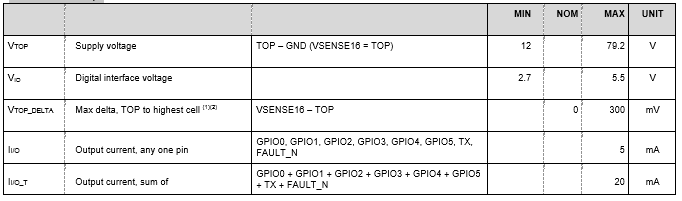
\includegraphics[width=\textwidth]{./img/BMS-operatingparms.png}
	\caption{Recomended operating parameters.}
	\label{fig:BMS-op-params}
\end{figure}


Each AMS board senses whole stack, that means it senses 144 cells, connected in 16s9p configuration. Comms wirings are protected by two 1kV 1nF capacitors CC1206KKX7RCBB102 by Yageo. There is placed one on each side (there is one on every AMS). The AMS is connected to Accumulator ECU that has capability of direct AIRs shutdown. The galvanic isolation between TS and GLV is done by two 1kV 1nF capacitors CC1206KKX7RCBB102 by Yageo. It is located on separated board connected between first AMS and Accumulator ECU.




\subsubsection{Accumulator indicator}
Describe the indicator, show wiring, provide tables with operation, PCB design, etc

\subsubsection{Wiring, cables, current calculations, connectors}
Describe the internal wiring, show schematics, provide calculations for currents and voltages and show data regarding the cables and connectors used.
\begin{itemize}
	\item 	Discuss maximum expected current, DC and AC how long will this be provided?
	\item Compare the maximum values to nominal currents
	\item Give a table for each kind of wire in your tractive-system:
	\item Describe your maintenance plugs, provide pictures
	\item Use tables like the one shown below:
\end{itemize}

% Table generated by Excel2LaTeX from sheet 'List1'
\begin{table}[htbp]
	\centering
	\caption{Wire data of company A, 0.205 mm$^2$.}
	\begin{tabularx}{\textwidth}{|X|X|}\hline
		Wire type &  \\[\TableSize]\hline
		Continuous current rating: &  \\[\TableSize]\hline
		Cross-sectional area &  \\[\TableSize]\hline
		Maximum operating voltage: &  \\[\TableSize]\hline
		Temperature rating: &  \\[\TableSize]\hline
		Wire connects the following components: &  \\[\TableSize]\hline
	\end{tabularx}%
	\label{tab:acc-wire}%
\end{table}%

\begin{figure}[H]
	\centering
	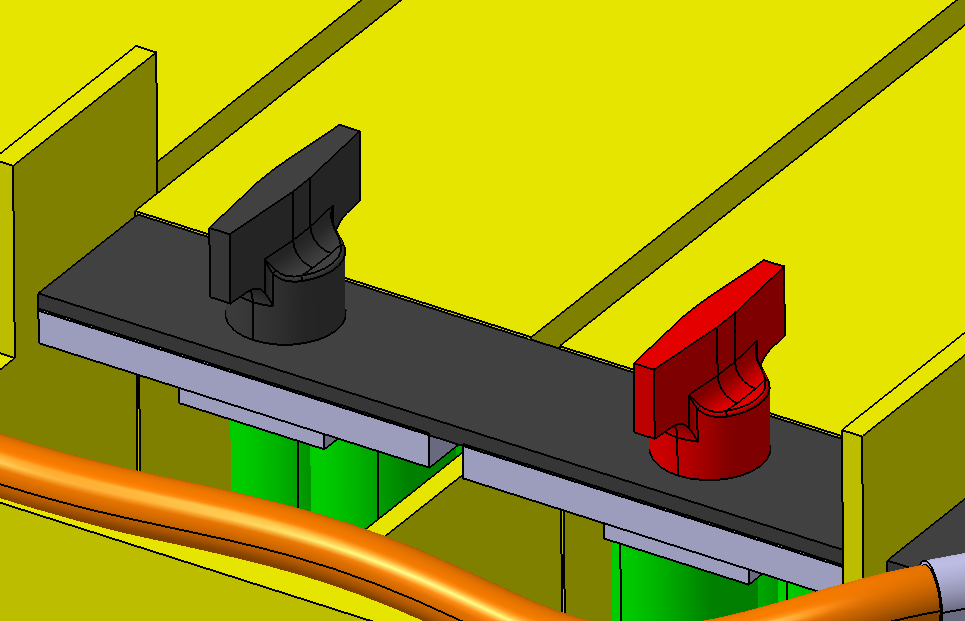
\includegraphics[width=\textwidth]{./img/ACP-nut.png}
	\caption{Maintance plugs I.}
	\label{fig:acp-maintance-plug}
\end{figure}

\begin{figure}[H]
	\centering
	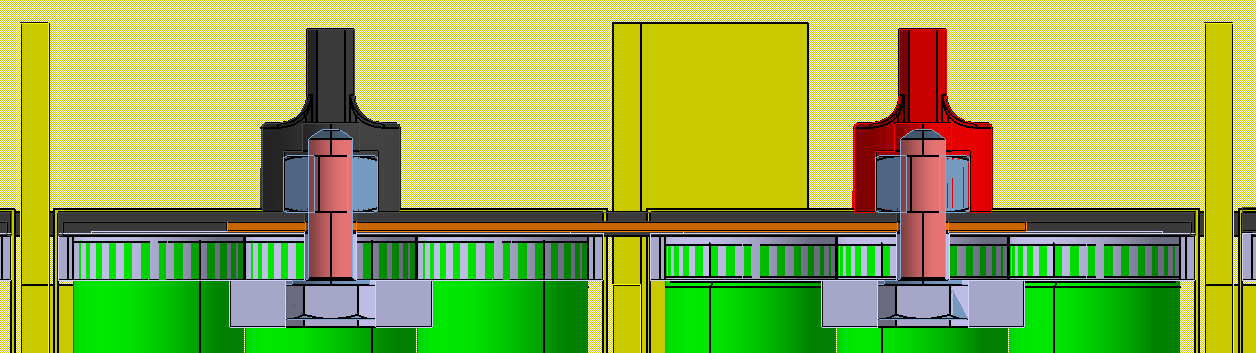
\includegraphics[width=\textwidth]{./img/ACP-nut2.png}
	\caption{Maintance plugs II.}
	\label{fig:acp-maintance-plug2}
\end{figure}

\begin{figure}[H]
	\centering
	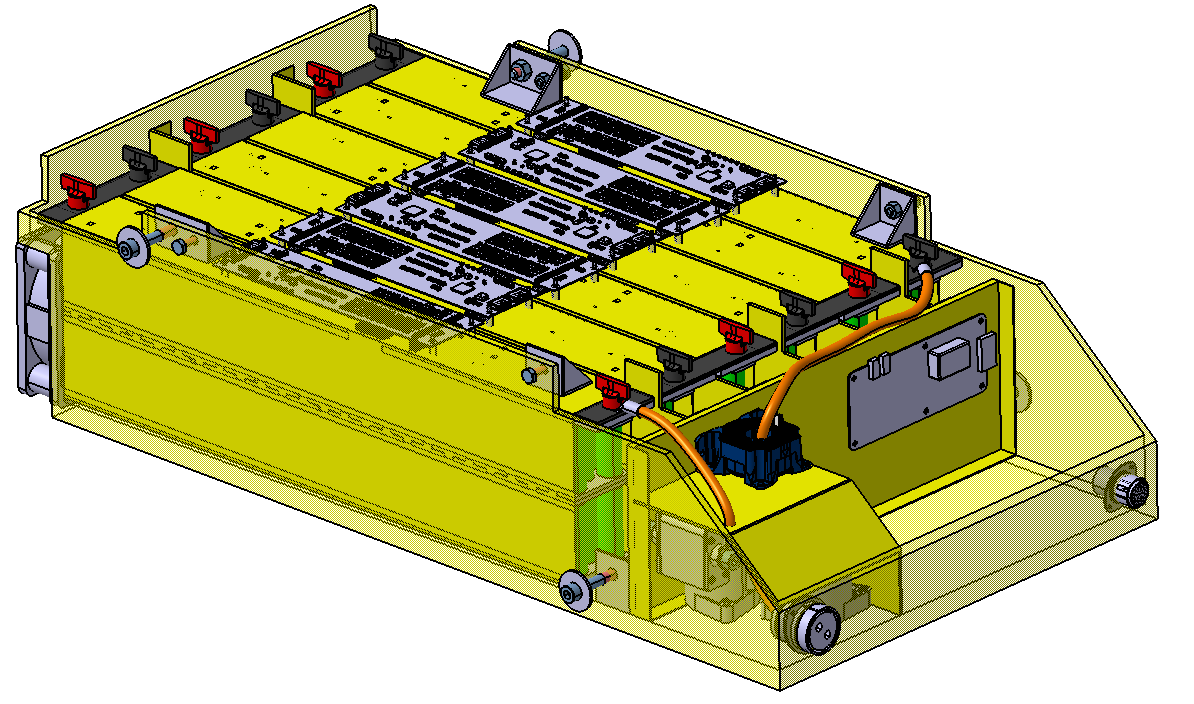
\includegraphics[width=\textwidth]{./img/ACP-view.png}
	\caption{Accumulator pack HV wiring I.}
	\label{fig:acp-hv-wiring}
\end{figure}

\begin{figure}[H]
	\centering
	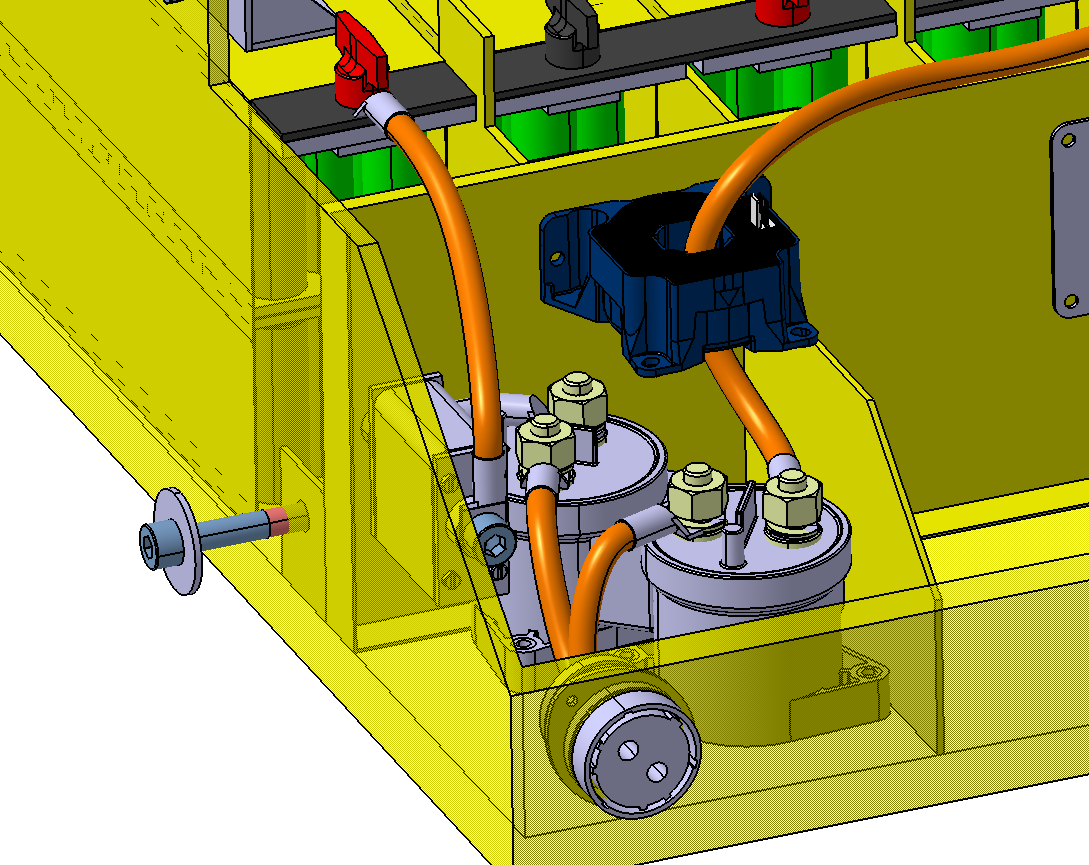
\includegraphics[width=\textwidth]{./img/ACP-fuse.png}
	\caption{Accumulator pack HV wiring II.}
	\label{fig:acp-hv-wiring2}
\end{figure}

\subsubsection{Accumualtor insulation relays}
Describe the AIRs used and their main operation parameters, use tables, etc.
Additionally, fill out the following table:

% Table generated by Excel2LaTeX from sheet 'List1'
\begin{table}[H]
	\centering
	\caption{Basic AIR data.}
	\begin{tabularx}{\textwidth}{|X|X|}
		\hline
		Relay Type: &  \\[\TableSize]
		\hline
		Contact arragment: &  \\[\TableSize]
		\hline
		Continous DC current rating: &  \\[\TableSize]
		\hline
		Overload DC current rating:  &  \\[\TableSize]
		\hline
		Maximum operation voltage: &  \\[\TableSize]
		\hline
		Nominal coil voltage: &  \\[\TableSize]
		\hline
		Normal Load switching: & \\[\TableSize]
		\hline
		Maximum Load switching &  \\[\TableSize]
		\hline
	\end{tabularx}%
	\label{tab:acc-air}%
\end{table}%

\subsubsection{Fusing}
Describe the fuses used and their main operation parameters, use tables, etc.
Additionally, fill out the following table for each fuse type used:

\begin{table}[H]
	\centering
	\caption{Basic fuse data}
	\begin{tabularx}{\textwidth}{|X|X|}
		\hline
		Fuse manufacturer and type: &  \\[\TableSize]
		\hline
		Continous current rating:  &  \\[\TableSize]
		\hline
		Maximum operating voltage  &  \\[\TableSize]
		\hline
		Type of fuse: &  \\[\TableSize]
		\hline
		I2t rating: &  \\[\TableSize]
		\hline
		Interrupt Current (maximum current at which the fuse can interrupt the current) &  \\[\TableSize]
		\hline
	\end{tabularx}%
	\label{tab:acc-fuse}%
\end{table}%

Create a table with components and wires protected by the fuse(s) and the according continuous current rating, below is an example table with some potential entries.  Complete this table with information for your design and add/remove additional locations as applicable.  Ensure that the rating of all the components is greater than the rating of the fuse such that none of the other components become the fuse.

% Table generated by Excel2LaTeX from sheet 'List1'
\begin{table}[H]
	\centering
	\caption{Fuse Protection Table}
	\begin{tabularx}{\textwidth}{|X|X|X|X|X|}
		\hline
		Location & Wire Size & Wire Ampacity & Fuse type & Fuse rating\\[\TableSize]
		\hline
		Cells to AIRs & 2 AWG & XXX & MNO Fuse & XXX \\[\TableSize]
		\hline
		AIR to Motor controller & 0 AWG & XXX & 2x MNO Fuse & XXX \\[\TableSize]
		\hline
		AIR to TSAL & 20 AWG & XXX & EFG Fuse & XXX \\[\TableSize]
		\hline
		Accumulator output connector & 2 AWG & XXX &     &  \\[\TableSize]
		\hline
		Cells to AMS &     &     &     &  \\[\TableSize]
		\hline
	\end{tabularx}%
	\label{tab:acc-fuse-protection}%
\end{table}%

\subsubsection{Charging}
Describe how the accumulator will be charged. How will the charger be connected? How will the accumulator be supervised during charging? Show schematics, CAD-Renderings, etc., if needed
Additionally, fill out the table:

\begin{table}[H]
	\centering
	\caption{General charger data}
	\begin{tabularx}{\textwidth}{|X|X|}
		\hline
		Charger Type: & \\[\TableSize]
		\hline
		Maximum charging power: &\\[\TableSize]
		\hline
		Maximum charging voltage: &  \\[\TableSize]
		\hline
		Maximum charging current: &  \\[\TableSize]
		\hline
		Interface with accumulator &  \\[\TableSize]
		\hline
		Input voltage: & \\[\TableSize]
		\hline
		Input current: &  \\[\TableSize]
		\hline
	\end{tabularx}%
	\label{tab:acc-charger}%
\end{table}%

\subsubsection{Mechanical Configuration/materials}
Describe the concept of the container, show how the cells are mounted, use CAD-Renderings, show data regarding materials used, etc.

\subsubsection{Position in car}
%Provide CAD-renderings showing the relevant parts. Mark the parts in the rendering, if necessary.  Ensure that the required mechanical structure to protect the accumulator and other electrical components is clearly identified.

\begin{figure}[H]
	\centering
	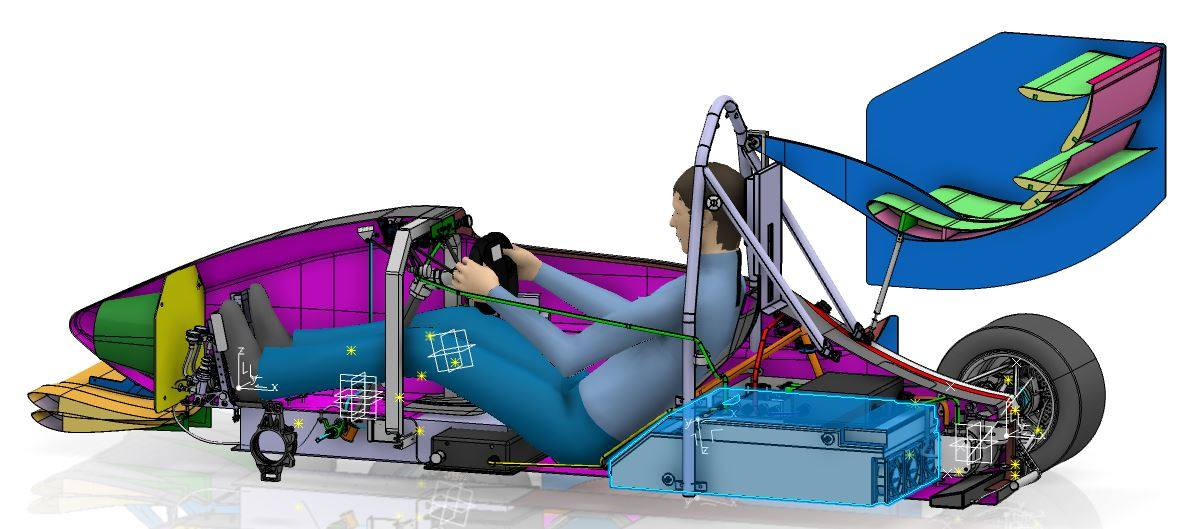
\includegraphics[width=\textwidth]{./img/acp-position.jpg}
	\caption{Position of ACP in car.}
	\label{fig:ACP-position}
\end{figure}





